\documentclass[11pt, oneside]{article}   	
\usepackage{geometry}                		
\geometry{letterpaper}                   		
\usepackage{graphicx}														
\usepackage{amssymb}
\usepackage{amsmath}
\usepackage[utf8]{inputenc}
\usepackage{float}

\title{Comprehensive Exam Notes}
\author{Patrick Dylan Barry}
						

\begin{document}
\maketitle
\abstract{}
During my Ph.D. at the University of Alaska Fairbanks I needed to study for comprehensive exams.
My committee made up of Anthony Gharrett, Megan McPhee, David Tallmon, and Eric Anderson 
were tasked with choosing topics that I needed to master in order to graduate and continue on the 
Ph.D. track. During my first committee meeting they made a list of topics: Relationship/Parentage analysis,
population genetic theory, coalescence, inference models for molecular ecology, population conservation 
genetics as applied to fisheries management, evolutionary ecology of Pacific salmon, and molecular genetic 
methodologies and applications. This list scared the bejezus out of me, and so I decided 
 that a good way of studying for these exams would be to create a short book that 
might aid in my preparation and be a good resource for the future. I think this should be worthwhile even
if nothing more grows out of this than a study guide for my exams or possibly lecture notes for a course I 
instruct. 
\newpage

\tableofcontents

\newpage

\section{A Brief History of the field of Genetics}
Hooke (1665) coins the term 'cell' after observing cellular structure in cork.

Anton van Leeuwenhoek (1670s) invents compound-like microscope - observes animalcules.

Schwann (1847) - proposes animals made of tissues which were constructed of 'cells'
Matthias Jakob Schleiden - plant cell structure - cells appear to be building blocks for complex organisms

Spontaneous generation
Redi - flies prevented from laying eggs = no maggots
Spallanzani - boiling hay infusion no animalcules
Pasteur and Tyndall - put it to rest
 
 Pangenesis -
 Aristotle eggs and sperm interact in mysterious way
 Hertwig used sea urchins to show developing embryo
 Strssburger did the same in plants - nucleus was important. 
 
 Fixity of Species - Linnaeus 
 
 Chromossomes - late 1800's 
 Boveri
 Henkens
 Montgomery
 
 Correns and deVries discover Mendels work. 

\section{DNA - a review}
In this section I will briefly review the discovery of DNA and review basic principles that will facilitate the 
understanding of preceding chapters. 
\subsection{DNA as the hereditary material}
Major experiments that lead to the discovery of DNA as the hereditary material. 
Biological molecule mediates inheritance. Possibilites - Carbohydrate/polysaccharide,lipid, protein, nucleic acid
Griffiths 1928
Dawson 1931
Alloway 1933
Avery, McCarty \& MacLeod 1944
Hershey\&Chase 1952
Fraenkel-Conrat and Singer 1957
Chargaff 1950
Linus Pauling
Watson/Crick/Franklin
\subsection{DNA structure}
Nucleotides - Nucleosides etc. 
\subsection{Transcription}
Brief description of DNA to mRNA
\subsection{Translation}
Brief description of mRNA to protein

\section{Molecular Genetic Methods \& Applications}

\subsection{Phenotypic Data}

\subsection{Codominant Phenotypic Data}

\subsection{Mitochondrial DNA (mtDNA)}
\subsubsection{History and Description}
Mitochondrial DNA (mtDNA) is, as its name suggests, DNA that is found within the mitochondria.
First described by Carl Benda in 1898, mitochondria are organelles found in most eukaryotic cells (plants, animals, and 
fungi) that generate adenosine triphosphate (ATP) from the phosphorylation of ADP through
cellular respiration. Details about the citric acid cycle (Krebs cycle) and the electron transport
chain which take pyruvate (the product of glycolysis) to produce ATP are covered in most 
introductory biology text books and are ommitted here. 

Nuclear and mtDNA have different evolutionary histories. It is theorized that mtDNA was derived from
the circular genome of an endosymbiotic bacteria ~1.5 billion years ago. This theory was first 
described by Schimper who in 1883 noticed striking similarties between chroplasts within green plants and 
freeliving cyanobacteria. The theory was later formalized by Mereschkowski, a Russian botanist, in 1910 and 
 further advanced by Lynn Margulis in 1967. 

Mitochondrial DNA is predominantly maternally inherited. There are a few explainations as to why
this is the case. Mere dilution might be responsible. The egg has upwards of 1,000,000 mtDNA molecules
while sperm have a high estimate of 1,000. The mtDNA on sperm is located on the tail to fuel the beating
of the flagellum. When the acrosome reaction occurs, the tail may not enter the egg effectively eliminating
the opportunity to pass on the male mtDNA. In 1999, it was reported by Sutovsky et al. that male
mtDNA is tagged with ubiquitin to mark them for later destruction in the embryo. 

Mitochonrial DNA in multicellular organisms is cirular and double stranded. In unicellular organisms mtDNA
is linearly organized DNA with telomeres and telemorase. In mammals, mtDNA encodes 37 genes (13 proteins, 
22 tRNAs, and the large and small subunits of the rRNA). The guanine rich strand, referred to
as the heavy strand (H-strand) encodes 28 genes, while the cytosine rich strand or light strand (L-strand)
endoceds the 9 other genes.  

\begin{figure}[H]
\begin{center}
    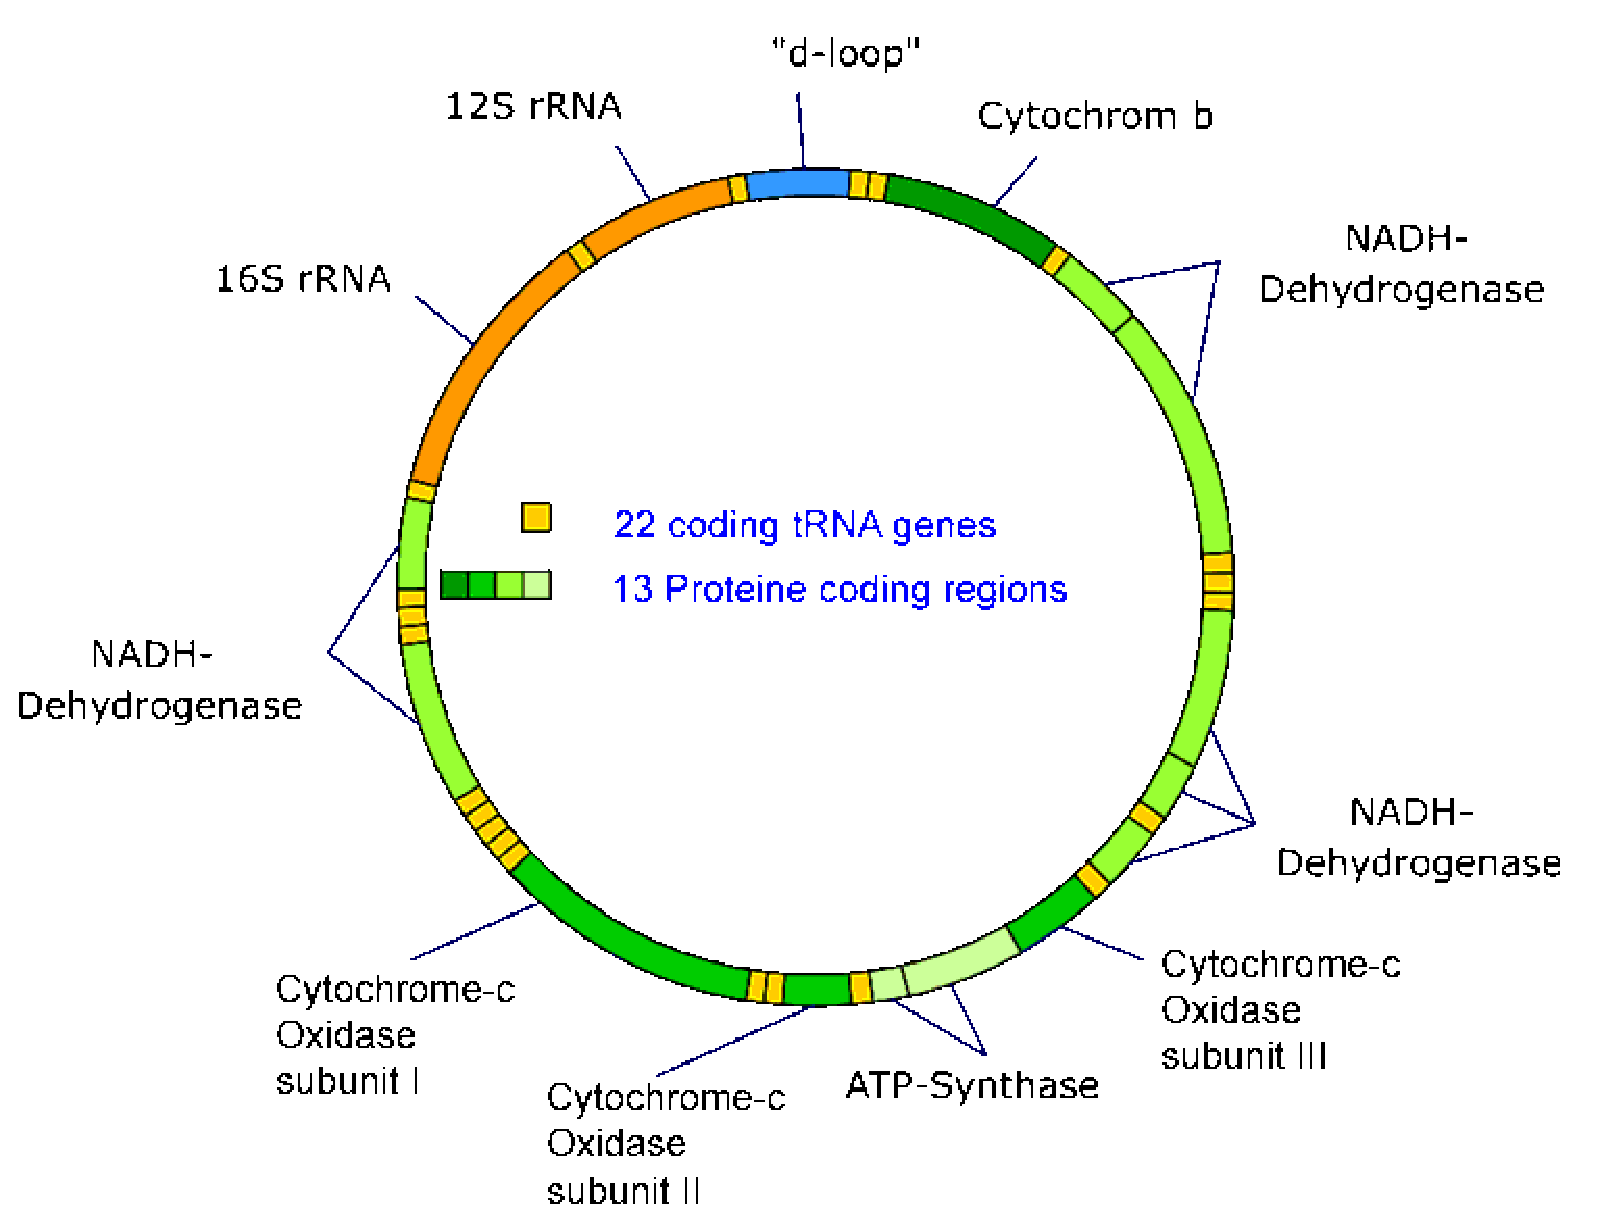
\includegraphics[width=25em]{images/mtDNA.pdf}   
    \caption{Structure of mammalian mtDNA molecule. The green segments represent the 13 protein genes,
the yellow segments are the tRNA genes, and the orange are the rRNA subunits.}
    \label{fig:mtDNA}
\end{center}
\end{figure}

\hrule

- 1970s to 1990 RFLP analysis of mtDNA dominated phylogenetics
- swtiched to DNA sequencing of mtDNA
- you can isolate mtDNA from other DNA by efficiently sparation of cytoplasm from cell nuclei.
Soft tissue is minced, homogenized and centrifuged at low speed (700 x g) to remove nuclei and cellular debris.
then centriguation at higher speed 20,000 x g pellets mitochondria.
CsCl-EtBr gradient centrifugation at speeds in excess of 160,000 x g makes mtDNA appear as a discete band 
that you can remove with a hypodermic needle and purify further with dialysis. 
- this was particularly fortuitous because organelle DNA can be transfered to the nucleus- sequences 
related to cytoplasmic genes now also exist as functionless derivaties in the nuclear genome 
Paralogous pseudogenes can wreak havoc on phylogenetic inference if they aren't accounted for. 

'control region' responsible for initiating replication and transcription.
variation exists in gene order and content useful in macrophylogeny. 

for the most part homoplasmic -> single mtDNA sequence predominates all cells of tissues in the 
organism



\hrule

\subsubsection{Use in phylogenetics and population genetics}
The analysis of mtDNA has been a mainstay of phylogenetics since XXXX and is still being used 

\subsection{Allozymes \& Isozymes}
Lacking the ability to look directly at the entire genome, early genetic studies relied on small bits of translated 
genomic regions. DNA is transcribed to mRNA which is then translated to protein (See Chapter 2). Consequently,
proteins represent a way of looking at variation within DNA sequences. Proteins are polypeptides 
composed of strings of amino acids joined by covalent peptide bonds. Mutations within the protein coding 
regions can lead to different amino acids being incorporated into the polypeptide. Two general types of enzymes 
have been studied extensively:  isozymes and allozymes.  \textbf{isozymes} are all functionally similar forms of 
enzymes. \textbf{Allozymes} are a subgroup of isozymes that are coded by a single locus. 
Their name is derived from \textit{all}ele (alternative forms of a gene) and en\textit{zyme}. Data collection for 
both types of marker rely on enzymatic reactions and staining so isozymes and allozymes can often be 
investigated simultaneously.
Gel electrophoresis allows proteins to be separated based on their physical properties: charge, size, and shape. 
This method exploits the porous properties of a starch or cellulose acetate gel matrix and the differential charge 
of the amino acids that make up the allozyme. The rate of movement on a gel, \textit{u}, is dependent on the net
protein charge \textit{Q}, shape {r}, strength of the electric field \textit{d} and viscosity of the suspension 
medium \textit{n}:

\begin{equation*}
u=\frac{Qd}{4\pi^2n}
\end{equation*}

Charge differences among allozymes are resultant of the 
differential incorporation of positive (basic at neutral pH) amino acids lysine (Lys), arginine (Arg) and 
histadine (His) and negative (acidic at neutral pH) amino acids aspartic acid and glutamic acid. 

The strength of allozymes 


Cons: only observe non-synonous mutations, only look at water soluble proteins, 
\subsection{Restriction Length Polymorphisms (RFLPs)}


\subsubsection{DNA barcoding}


\subsection{Microsatellites \& Minisatellites}

\subsection{Sequencing}
\subsubsection{Sanger Method}
Who developed it, how it was done, pros\&cons
\subsubsection{Pyrosequencing}
Who developed it, how it was done, pros\&cons
\subsubsection{RADsequencing}
Who developed it, how it was done, pros\&cons

\subsection{Single Nucleotide Polymorphisms (SNPs)}
Who developed it, how it was done, pros\&cons
\subsubsection{Genotyping by sequencing}


\end{document}  